% !TEX root = ../thesis.tex

\chapter{Introduction}
\label{chapter:introgen}

Recent years have seen enormous advances in the field of cosmology. Thanks to technological advancements, wide-field galaxy surveys have helped mapping the universe, and in particular have provided high-precision data on the distribution of galaxies. From the earliest realisations that these observed galaxies can be used to trace the underlying matter density fields, the field of large-scale structure research has been transformed into a data-driven science. 

Next-generation surveys will be able to observe the large scale structure of galaxies at unprecedented precision. To make the most of this wealth of high-precision cosmological data, our theoretical description must match experimental precision. The work in this thesis was undertaken as an effort to extend the theoretical description of the galaxy bispectrum, which will be a key probe in future large scale surveys. On these scales a variety of relativistic effects come into play once the observed number-count fluctuation is projected onto the past lightcone. These effects need to be accounted for properly in order for them to not bias measurements of primordial non-Gaussianty and other cosmological parameters.
To start, in this chapter we will introduce the standard cosmological model, $\Lambda$CDM, and briefly discuss the observational evidence supporting the standard model of cosmology. We also discuss structure formation in the universe, and introduce galaxy statistics, which has been the crucial tool for studying the clustering of galaxies in the universe. Up to now, the two-point correlation function, or power spectrum in Fourier space, has been a cosmologist's most reliable statistic describing the LSS and constraining cosmological parameters. We will give a brief overview of what has been achieved with the power spectrum, and introduce the galaxy bispectrum as the first of the higher-order correlation functions. 

\section{The standard cosmological model}

Over the past several decades, a consensus model for describing the evolution of the universe has emerged.  Evidence for this model is provided by a variety of observations, made possible due to technological advancements, such as the measurements of the cosmic microwave background (CMB), distance measurements using Type 1a Supernovae (SNe) and the BAO, and large-scale structure surveys. 

This standard model for the evolution of the universe predicts that approximately 13.8 billion years ago, the universe was in a hot and dense `Big Bang' state, from which it has continued to expand since. From Type 1a SNe measurements, it has been inferred that the late-time expansion of the universe is accelerating due to an energy component referred to as `dark energy', the physical origin of which has not yet been understood, but described by the cosmological constant, $\Lambda$. Approximateley 70\% of the universe's energy budget at the present day is comprised of this dark energy. The remaining amount primarily consists of `cold dark matter' (CDM), a collisionless component which makes up about 25\% of the universe's energy content. The small remaining amount is comprised of roughly 4\% of the more familiar baryonic matter, which interacts electromagnetically, and a small relativistic radiation component (photons and neutrinos). See figure~\ref{fig:contentuniverse} for an illustration of the energy components of the universe at present day. It is from these dominant energy components that the colloquial name of the standard cosmological model is derived-- it is referred to as $\Lambda$CDM.
\begin{figure}[ht]
	\centering
	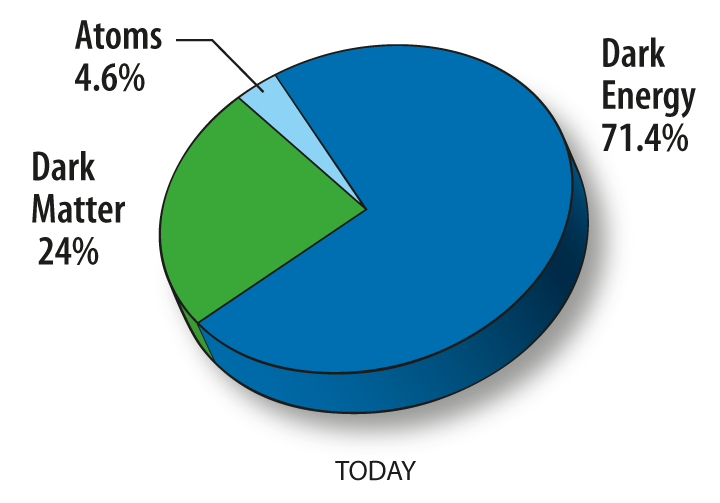
\includegraphics[width=0.6\textwidth]{fig/placeholer_energycontent_wmap.png}
	\caption{An illustration (will replace with similar illustration I make myself) of the modern-day dominant energy components in the universe.}
	\label{fig:contentuniverse}
\end{figure}

\begin{figure}[ht]
	\centering
	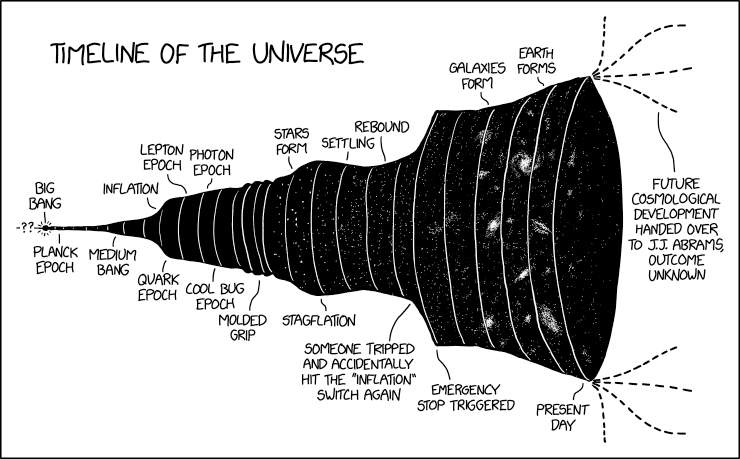
\includegraphics[width=0.8\textwidth]{fig/timeline_of_the_universe.png}
	\caption{Picture of timeline of universe - replace with serious one}
	\label{fig:timelineuniverse}
\end{figure}
In the 1980's, the theory of inflation was coined~\cite{Guth:1980zm,Linde:1981mu,Albrecht:1982wi}, which has since become the prevailing theory for the early universe and its initial conditions. As a theory, it aims to solve the horizon, flatness, homogeneity and isotropy problems. During inflation, the universe is expanding exponentially, rapidly increasing its scale by a factor of at least $\approx 10^{27}$. During this period of exponential expansion, quantum fluctuations are stretched to macroscopic level. These are the seeds of the cosmic structure we observe today. It is worth noting that while the properties of the universe (near homogeneous, isotropic, and spatially flat) as predicted by inflation have been confirmed observationally, but as of yet there is no conclusive observational evidence for the inflationary model itself. 

After inflation ends, the universe cooled down, and keeps expanding though at a much slower rate than it did before. The thermal evolution of the universe is defined by the `competition' between the interaction rates of the particles and the expansion rate of the universe itself. The baryonic mass of the universe consists of approximately 75\% hydrogen ions and 25\% helium ions, plus small amounts of deuterium and lithium, all of which are created through Big Bang nucleosynthesis. Electrons and neutrinos are also present, and the charged baryonic matter is tightly coupled by electromagnetic interaction. Furthermore, the free electrons are tightly coupled also, to the photons, via Thompson scattering. All of this results in the so-called photon-baryon fluid. The pressure of this fluid prevents the fluctuations from gravitationally collapsing, which leads instead to the generation of acoustic waves. These are known as the Baryon Acoustic Oscillations (BAO), propagating until the protons and baryons decouple. This occurs around the time of `recombination' around 400,000 years after the Big Bang. At recombination, the universe has cooled down sufficiently for neutral hydrogen to form, and the now decoupled photons can free stream from the `surface of last scattering' through the universe. This background radiation, the `first light' of the universe, can be observed today and has a temperature of about 2.7 K-- it is known as the Cosmic Microwave Background (CMB), and primordial fluctuation patterns are imprinted on the temperature fluctuations of the CMB. 

Around 50,000 years after the Big Bang, and after a period of radiation domination, the universe becomes dominated by its matter content. This matter dominated era lasts for about 10 billion years. Under matter domination, the primordial density fluctuations grow due to gravitational instability. This gravitational collapse eventually leads to the formation of the cosmic web, which is a non-linear structure formed by halos, voids, and filaments, dominated by CDM. See figure~\ref{fig:millennium} for a snapshot from simulations of the cosmic web. 

\begin{figure}[ht!]
	\centering
	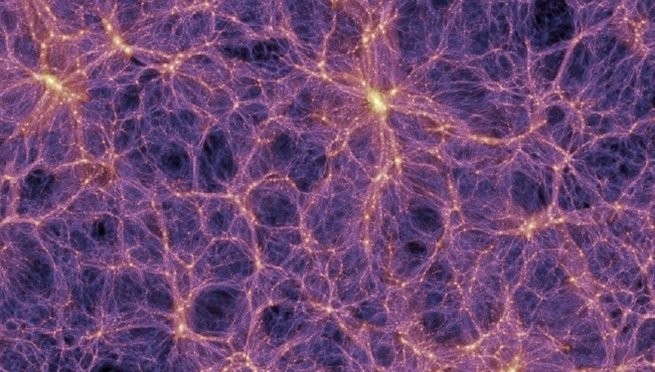
\includegraphics[width=0.8\textwidth]{fig/Millennium.png}
	\caption{Snapshot of Millennium simulations~\cite{Springel:2005nw} showing non-linear LSS. There are dense filaments (lighter) surrounded by milder underdensities (darker). }
	\label{fig:millennium}
\end{figure}

Baryonic matter inside these dark matter halos cools down, collapses, and goes on to form stars and galaxies. Formation of this large scale structure is hierarchical, as smaller objects form first and merge to into larger structures. The resulting evolution of structure can be well-described by a linear description of perturbations on large scales (of about 150Mpc), but the small-scale nonlinearities of the fluctuations pose serious theoretical challenges.

In the standard $\Lambda$CDM model, the universe is assumed to be spatially flat, and its evolution is described by six parameters-- the present-day baryon and cold dark matter densities, the angular size of the sound horizon, the optical depth due to reionisation, the scalar power spectrum index, and the amplitude of the primordial curvature perturbations. The current best constraints on these parameters are given in table~\ref{tab:planck2018params}.

\begin{table}[ht]
	\centering
\begin{tabular}{ l | l}
	\textbf{Parameter} & \textbf{Value} \\
	\hline
	$\Omega_b h^2$ & $0.02242 \pm 0.00014$ \\
	$\Omega_c h^2$  & $0.11933 \pm 0.00091$ \\
	$100 \theta_\star$ & $1.04101 \pm 0.00029$ \\
	$\tau$  & $0.0561 \pm 0.0071$ \\
	$n_s$  & $0.9665 \pm 0.0038$ \\
	$\ln (10^{10} A_s)$  & $3.047 \pm 0.014$
\end{tabular}
	\caption{Planck 2018 best-fit parameters in the standard, spatially flat, $\Lambda$CDM model~\cite{Aghanim:2018eyx}. The tabulated parameters are from top to bottom the baryon density ($\Omega_b h^2$), the CDM density ($\Omega_c h^2$), the angular size of the sound horizon ($100 \theta_\star$), the optical depth due to reionisation ($\tau$), the scalar power spectrum index ($n_s$), and the amplitude of primordial curvature perturbations ($\ln (10^{10} A_s)$).} \label{tab:planck2018params}
\end{table}

Support for the $\Lambda$CDM model comes from a variety of observational probes. The anisotropies of the CMB as measured by the WMAP~\cite{Bennett:2013} and Planck~\cite{Aghanim:2018eyx} satellites, and the ground-based telescopes Atacama Cosmology Telescope~\cite{Das:2013zf} and South Pole Telescope~\cite{George:2014oba}, which have all supplied strong constraints on matter and radiation densities, the angular diameter distance to the surface of last scattering, and the shape and the amplitude of the primordial power spectrum. The BAO features have been measured successfully by galaxy redshift surveys on scales of about 150 Mpc. This BAO feature is the imprint of the acoustic waves in the baryon-photon fluid onto the clustering of density field tracers. Measurements of the BAO have provided constraints on the expansion rate of the universe across a wide range of different redshifts~\cite{BOSS:2016wmc,Ross:2014qpa,Oka:2013cba,Sanchez:2006,Beutler:2011,Kazin:2014qga}. Furthermore, Type 1a SNe have yielded the first evidence for dark energy~\cite{SupernovaSearchTeam:1998fmf,SupernovaCosmologyProject:1998vns}, as well as complementary constraints on the expansion rate of the universe and the value of the present-day Hubble parameter $H_0$~\cite{Freedman:2012,Riess:2016jrr,Suzuki:2012,SDSS:2014iwm}. Further constraints on the growth of structure obtained from weak gravitational lensing~\cite{DES:2017qwj,Heymans:2013fya} and RSD analyses of anisotropic clustering measurements~\cite{BOSS:2016psr,BOSS:2016teh}. All these observations considered together provide compelling evidence for the $\Lambda$CDM model.

\section{Observing large scale structure}

As described previously, the most natural explanation for the formation of the large scale structure of the universe as observed in galaxy surveys is for them to be the result of amplification of the primordial fluctuations due to gravitational interaction of cold dark matter. Already before the detailed observations of the CMB anisotropies that reveal the imprint of the stretched-out primordial fluctuations, it was known that the galaxies in our universe are not randomly distributed. The first detections of this structure on larger scales was through a variety of galaxy surveys that aimed to observe and map the distribution of galaxies in the local universe. This all started off with Hubble's first detections of inhomogeneities in the early 20th century, at the time incorrectly thought to be `spiral nebulae'~\cite{Hubble:1926,Hubble:1934}. Following this, advancements in cosmology have been primarily held back by lack of sufficient technological progress to carry out precision surveys at large scales, until the publication of larger galaxy catalogues in the 1960's~\cite{Shane:1967,Zwicky:1961}. Around the same time, theoretical modelling advanced with the realisation that galaxies could be used as biased tracers of the underlying dark matter density field. A series of important papers followed, from systematic analysis of galaxy catalogues~\cite{Peebles:1973} to the first cosmological inferences from LSS data~\cite{Zeldovich:1970,Davis:1977mar,Davis:1977aug,Davis:1983,Peebles:1980,Maddox:1990,Baumgart:1991,Park:1992}. 

Technological advancements, allowing for larger and more precise datasets, made further theoretical progress possible. Interpretations of clustering results gave rise to a new field of study known as galaxy bias, studying the relationship between the galaxies and the underlying dark matter\cite{Davis:1985,Rees:1985,Cole:1989vx,Kaiser:1984}-- a brief overview of the relevant local model of galaxy bias for the purpose of this thesis is given in section~\ref{section:galaxybias}. Peculiar velocities of galaxies were found to influence observations of clustering, which lead to several important publications on redshift-space distortions~\cite{Kaiser:1987qv,Davis:1983,Hamilton:1992zz}. These in turn were significant for the early redshift surveys~\cite{Cole:1994wf,Loveday:1995gk,Tadros:1999ky}. The early analyses also provided some of the earliest evidence for the $\Lambda$CDM model, by showing that the then-prevailing theory of a flat, matter-dominated universe did not explain the observed clustering data.

\begin{figure}[!ht]
	\centering
	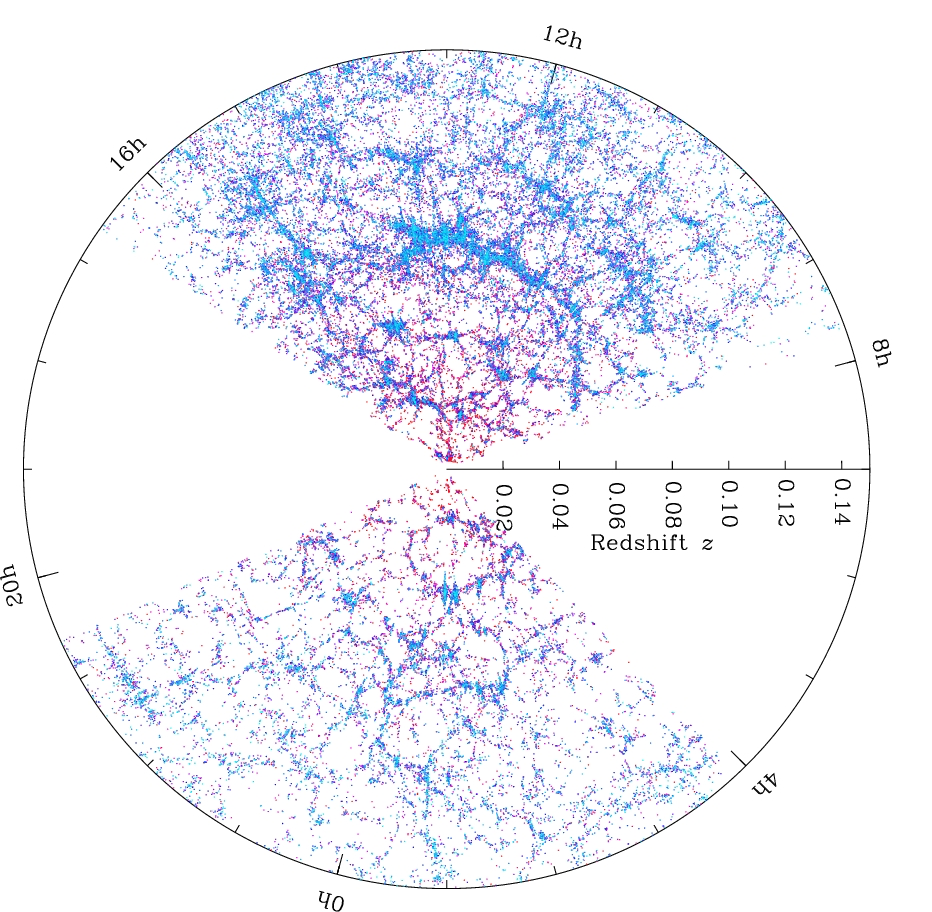
\includegraphics[width=0.8\textwidth]{fig/sdss.png}
	\caption{Example sky map of a redshift survey, with the cosmic web at increasing redshift. This figure is adapted from the SDSS Science Results~\cite{SDSS:2018ws}.}
	\label{fig:redshiftsurveypicture}
\end{figure}

Accurate redshift measurements made possible by the rise of new multi-fiber spectrograph technology allowed for redshift-space mapping of hundreds of thousands of objects. Pioneering surveys in this field are the Two-degree Field Galaxy Redshift Survey (2dFGRS)~\cite{2DFGRS:2001zay} and the Sloan Digital Sky Survey~\cite{SDSS:2000hjo}-- see Figure~\ref{fig:redshiftsurveypicture} for an example of the large scale structure as measured by these redshift surveys.

Measurements of the BAO in galaxy clustering surveys can help optimise constraints on the expansion rate and on properties of dark energy. The Baryon Acoustic Oscillation Survey (BOSS)~\cite{Dawson:2012} has yielded a dataset with redshift measurements for more than 1.5 million galaxies, with redshifts ranging from $0.2 < z < 0.75$ which has resulted in percent-level constraints on the expansion rate in this redshift range~\cite{BOSS:2016wmc}. These constraints are complemented at lower redshift by results from the 6dF Redshift Survey~\cite{Beutler:2011} and at higher redshift by the WiggleZ survey~\cite{Blake:2011a,Blake:2011b}. 

There remains a number of unanswered questions in cosmology and LSS, for example finding out more about the origin of cosmic acceleration, and studying the physics of the early universe, which includes detection of primordial non-Gaussianity. Such a detection could help discriminate between various theories of inflation and other models of the early universe. The current state-of-the-art surveys are the so-called Stage III surveys, and they include eBOSS~\cite{Dawson:2015wdb}, the Dark Energy Survey (DES)~\cite{DES:2014xto}, and the Hobby-Eberly Telescope Dark Energy Experiment (HETDEX)~\cite{Hill:2008}. 
The next-generation surveys, which will provide us with a wealth of high precision cosmological information, are known as Stage IV surveys. These include e.g. the Dark Energy Spectroscopic Instrument (DESI\footnote{https://www.desi.lbl.gov}), the Subaru Prime Focus Spectrograph (PFS\footnote{https://pfs.ipmu.jp}), 4MOST\footnote{https://www.4most.eu/cms/}, LSST on the Vera Rubin Telescope\footnote{https://www.lsst.org}, the space-based instruments Nancy Grace Roman Space Telescope\footnote{https://roman.gsfc.nasa.gov} (formerly WFIRST) and Euclid\footnote{https://www.euclid-ec.org}, and 21cm intensity mapping surveys MeerKAT\footnote{www.sarao.ac.za/science/meerkat/}, the SKA\footnote{{www.skatelescope.org/}}, and HIRAX\footnote{hirax.ukzn.ac.za/}. 

In this thesis, we treat two surveys with specific interest. The first is a Stage IV spectroscopic galaxy survey similar to what will be carried out by the Euclid satellite. Secondly, we consider in more detail the use of intensity mapping of 21cm emission as a tracer of the galaxy distribution in cosmology, such as the SKA, HIRAX, and PUMA (the latter of which is still in proposal stage). These surveys are discussed in more detail in Chapter~\ref{chapter:detect}. 


\section{Statistics of galaxy clustering}
\label{section:introbisp} 


\iffalse
Tests of theories of the early universe that describe the primordial fluctuations are statistical in nature for a number of reasons. For one, there is no direct observational access to primordial fluctuations, and secondly, the timescales required to follow cosmological evolution of systems is much longer than that over which observations are realistically possible. In essence this means that observations on the past lightcone show different objects at different phases of their evolution, and as a result, tests of the evolution of large scale structure must be carried out statistically. 
\fi

A goal of theoretical cosmology is to make statistical predictions which depend on the statistical properties of primordial perturbations, which in turn lead to the formation of large scale structures in the universe. In these models, the observable universe is modelled simply as a stochastic realisation of a statistical ensemble of possibilities. The most widely considered models are based on the inflationary paradigm, and the simplest (single-field slow-roll) models generally give rise to adiabatic Gaussian initial fluctuations. In this case, the origin of stochasticity lies in quantum fluctuations that were generated in the early universe. 

In a LSS galaxy survey, the fluctuations in the number of galaxies are measured and mapped across the sky. Such a galaxy map can be pixelised in bins in solid angle and redshift. If we observe in some observed direction $\n$ and at some redshift $z$, we count the number of galaxies in a bin of size $dz$ and solid angle $d\Omega$ centered at this $(\n,z)$, which gives the observed angular number density of galaxies $N(\n,z)$. The mean angular number density at each redshift, $\bar{N}(z)$, can be obtained by averaging over all observed directions $\n$. \iffalse
\begin{equation}
	\diff \bar{N} = N \diff z \diff \Omega\,.
\end{equation} \fi
 Then, the galaxy number count fluctuation is defined simply by, 
\begin{equation}
	\delta_g(\n,z) = \frac{N(\n,z) - \bar{N}(z)}{\bar{N}(z)}\,.
\end{equation}
We will briefly review some of the results that have been obtained from studying the two-point correlation function of $\delta_g(\n,z)$. A purely Gaussian field would be fully described by the two-point correlation, which is the joint ensemble average of the density fluctuation at two different points. However, one of the primary goals of next-generation surveys is to detect primordial non-Gaussianity, and for this to be possible, theoretical accuracy must match experimental precision. This gives rise to the need for analysis of higher-order correlators, which will contain information that is both complementary and additional to what is contained in the power spectrum. The first of these higher-order correlation functions is the three-point function or bispectrum. The bispectrum will be crucial for helping improve constraints in future surveys, and the remainder of this thesis is concerned with improving the theoretical description of the bispectrum of galaxies, as well as exploring the feasability of detecting such a signal in upcoming surveys.

\subsection{The two-point function}

A purely Gaussian field is fully described by the two-point correlation function or power spectrum. The two-point correlation function is defined as the joint ensemble average of the density at two different points $\x$ and $\x + \textbf{r}$, i.e. 
\begin{equation}
	\xi(r) = \langle \delta(\x) \delta(\x + \textbf{r}) \rangle,
\end{equation}
which is dependent on the distance $r$ between the two points only, due to statistical homogeneity and isotropy which are assumed throughout. Usually, the density contrast $\delta$ is expressed in terms of its Fourier space components.

\iffalse, where our Fourier convention is 

\begin{equation}
	\delta({\x}) = \int \frac{\diff^3k}{(2\pi)^3} \, e^{\i \k \cdot \x } \delta(\k),
\end{equation}
where $\delta(\k)$ are complex random variables. Note that there are other Fourier conventions in use in literature, which differ as to where the factors of $2\pi$ go. \fi

Since the density contrast is real, this means that we have
\begin{equation}
	\delta(\k) = \delta^*(-\k).
\end{equation}

Similarly, the correlators can also be computed in Fourier space, as follows, 
\begin{equation}
	\langle \delta(\k) \delta(\k') \rangle = \int \diff^3 x \diff^3 r \, \langle \delta(\x) \delta(\x + \r)\rangle e^{-\i (\k + \k') \cdot \x - \i \k' \cdot \r}.
\end{equation}
This can be rewritten using the definition of the two-point correlation function as 
\begin{equation}
	\langle \delta(\k) \delta(\k') \rangle = \int \diff^3 x \diff^3 r \, \xi(r) e^{-\i (\k + \k') \cdot \x - \i \k' \cdot \r},
\end{equation}
and, performing one of the integrals, 
\begin{align}
	\langle \delta(\k) \delta(\k') \rangle &= (2\pi)^3 \delta^D(\k + \k') \int \diff^3 r \,\xi(r) e^{\i \k \cdot \r} \\
	&\equiv (2\pi)^3 \delta^D(\k + \k') P(k),
\end{align}
where $P(k)$ is by definition the (density) power spectrum. There are several cosmology codes available for simulation the evolution of linear perturbations in the universe and computing LSS observables-- most well known are Class (Cosmic Linear Anisotropy Solving System,~\cite{Lesgourgues:2011}) and CAMB (Code for Anisotropies in the Microwave Background,~\cite{Lewis:1999bs}), both of which are used to generate power spectra and other quantities used in numerical results in this thesis. An example of a power spectrum generated with CAMB is given in figure~\ref{fig:powerspectrum}.
\begin{figure}[!ht]
	\centering
	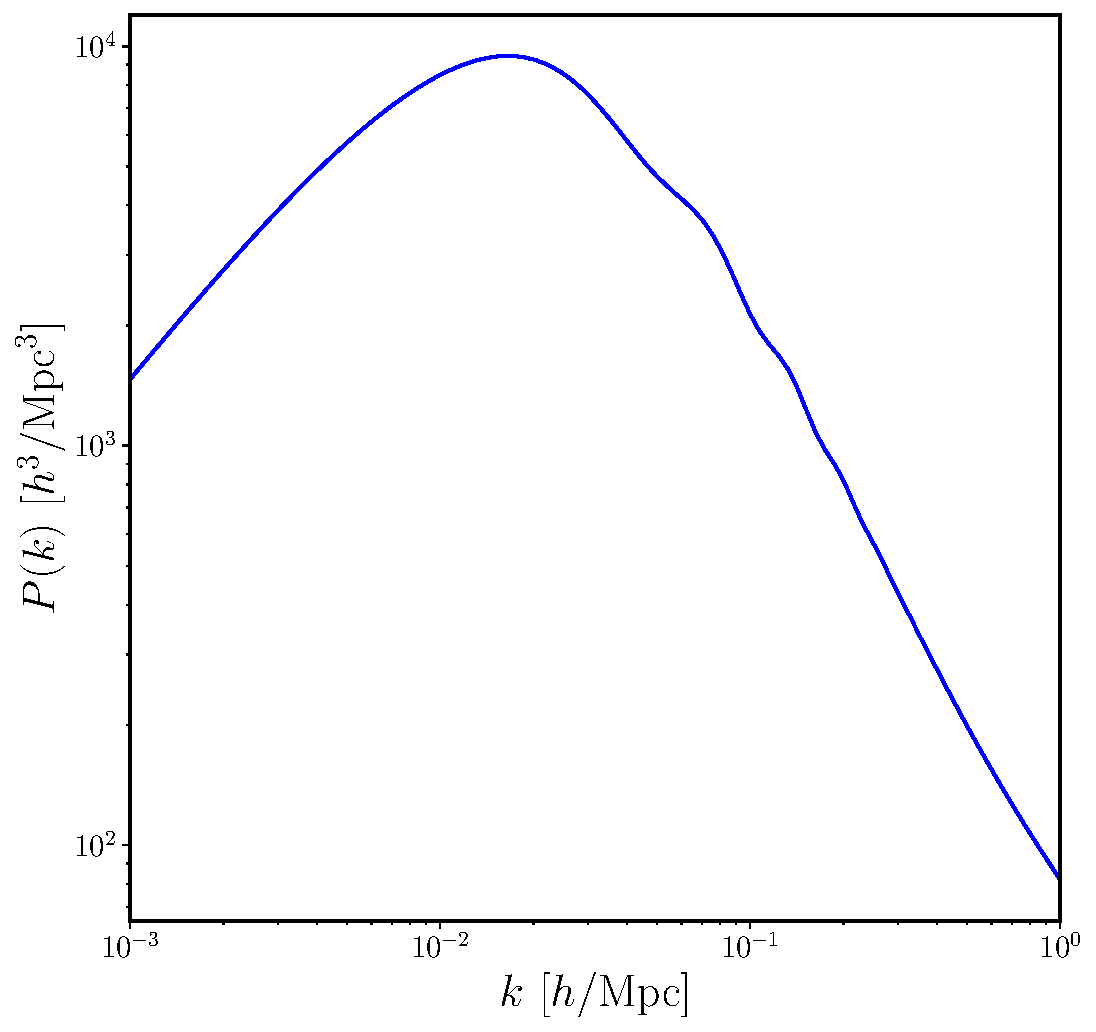
\includegraphics[width=0.7\textwidth]{fig/matterpower_z1.pdf}
	\caption{Example of a linear matter power spectrum as generated by CAMB, at redshift $z=1$.}
	\label{fig:powerspectrum}
\end{figure}

The galaxy power spectrum has been used extensively to extract cosmological information from large scale surveys. However, the observed distribution of galaxies has several more complex features, such as e.g. compact clusters, and underdense regions. These features are not captured by two-point statistics, which means that especially when more precise measurements are carried out such as will be the case for the next generation of surveys, information would be lost. This gives rise to the need for higher-order statistics and their Fourier transforms. 

\subsection{The three-point function}

\subsubsection{Construction of higher-order correlators}

Higher-order correlation functions are defined as the connected part of the joint ensemble average of the density in an arbitrary number of locations. In principle, it is possible define any order of correlation function like this, but they will rapidly become more computationally complex and expensive. In the case of a purely Gaussian field, the only non-vanishing connected part is the two-point correlation function. This is a direct consequence of Wick's theorem for Gaussian fields, and has a number of important consequences. Firstly it means that a purely Gaussian, statistically homogeneous and isotropic field is fully described by its two-point correlation function or power spectrum, and secondly it means that the statistical properties of any field, which is not necessarily linear, can be written in terms of combinations of two-point correlation functions -- as long as the field is built from a Gaussian field $\delta$. In a generic form, Wick's theorem can be expressed as 
\begin{align}
	&\langle \delta(\ka) \ldots \delta(\bm{k}_{2p + 1}) \rangle = 0 \nonumber \\
	&\langle \delta(\ka) \ldots \delta(\bm{k}_{2p})\rangle = \sum_{[\text{all distinct pairs}]} \prod_{[p \text{ pairs } (i,j)]} \langle \delta(\bm{k}_i) \delta(\bm{k}_j) \rangle.  
\end{align}

More concretely, this means that for a purely Gaussian field, $\langle \delta(\ka) \delta(\kb) \delta(\kc)\rangle = 0$. However, this changes in the presence of any sources of non-linearity. An important consequence of non-linear evolution of structure is that the statistics of odd-number density fields are no longer vanishing. The leading odd-number statistic which will be non-zero in the case of non-linear evolution if the three-point correlation function or the bispectrum in Fourier space, 
\begin{equation}
	\langle \delta(\ka) \delta(\kb) \delta(\kc) \rangle = (2 \pi )^3 \delta^\mathrm{D}(\ka + \kb + \kc) \left[ 2 F_2(\ka,\kb) P(\ka) P(\kb) + \text{ 2 c.p.} \right]
\end{equation}
where $F_2$ is the Fourier space density evolution kernel, which is given by, 
\begin{equation}
	F_2(\ka,\kb) = 1 + \frac{F}{D^2} + \left( \frac{k_1}{k_2} + \frac{k_2}{k_1} \right) \ka \cdot \kb + \left( 1 - \frac{F}{D^2} \right) \left( \ka \cdot \kb \right)^2\,,	
\end{equation}
where $F \equiv F(a)$ is the second-order growth factor, and the Einstein-De Sitter relation $F/D^2 = 3/7$ is a very good approximation for $\Lambda$CDM. Further, $P$ is the linear power spectrum from the previous discussion, and redshift dependence is suppressed for brevity. More generally, we can write, 
\begin{equation}
	\langle \delta(\ka) \delta(\kb) \delta(\kc) \rangle = (2 \pi )^3 \delta^\mathrm{D}(\ka + \kb + \kc) B_g(\ka,\kb,\kc)\,,
\end{equation}
where redshift dependence is suppressed once again, and $B_g$ is the galaxy bispectrum, dependent on direction and moduli of the three wavevectors, and roughly proportional to $P(k)^2$ in amplitude.


\subsubsection{The Fourier-space bispectrum}

As the bispectrum is a non-Gaussian statistic, and as such is especially sensitive to any forms of non-linearity in the universe. It is an essential probe for e.g. primordial non-Gaussianity in next-generation surveys. There are other sources of non-Gaussianity in the universe, for example gravitational instability on small scales. Primordial non-Gaussianity, which is often parametrised by the non-linear parameter $\fnl$, is predicted by different types of inflation and other theories of the early universe; meaning that improvement of constraints on $\fnl$ could help discriminate between these theories and help shed light on the very early universe and the seeds of structure formation. 

The bispectrum in Fourier space forms a closed triangle correlating three different wave-vectors and, unlike the power spectrum or two-point function, is able to correlate different scales. The matter bispectrum is unique from the thus far more well-studied CMB bispectrum in that it is able to form a three-dimensional map of the universe, whereas the cosmic microwave background provides a two-dimensional snapshot of the first light only. It is therefore essential to try and improve the theoretical description of the matter bispectrum if we are to utilise the wealth of information from next-generation high-precision galaxy surveys in as good and as unbiased a manner as possible. 

Similar to how the power spectrum is a measure of probability of finding pairs of galaxies at a given separation from each other, the bispectrum analogously maps this to a probability in a three-dimensional equivalent. That is, it can correspond directly to the filamentary structure formed by matter and voids which we know as the cosmic web. The bispectrum has degrees of freedom in both modulus of the wavevector i.e. scales of correlation, as well as the shape of the triangle itself. See figure~\ref{fig:realspacesignature} for an example of how a given triangle shape in Fourier space translates to a real-space structure of overdensities and voids. 

\begin{figure}[ht!]
	\centering
	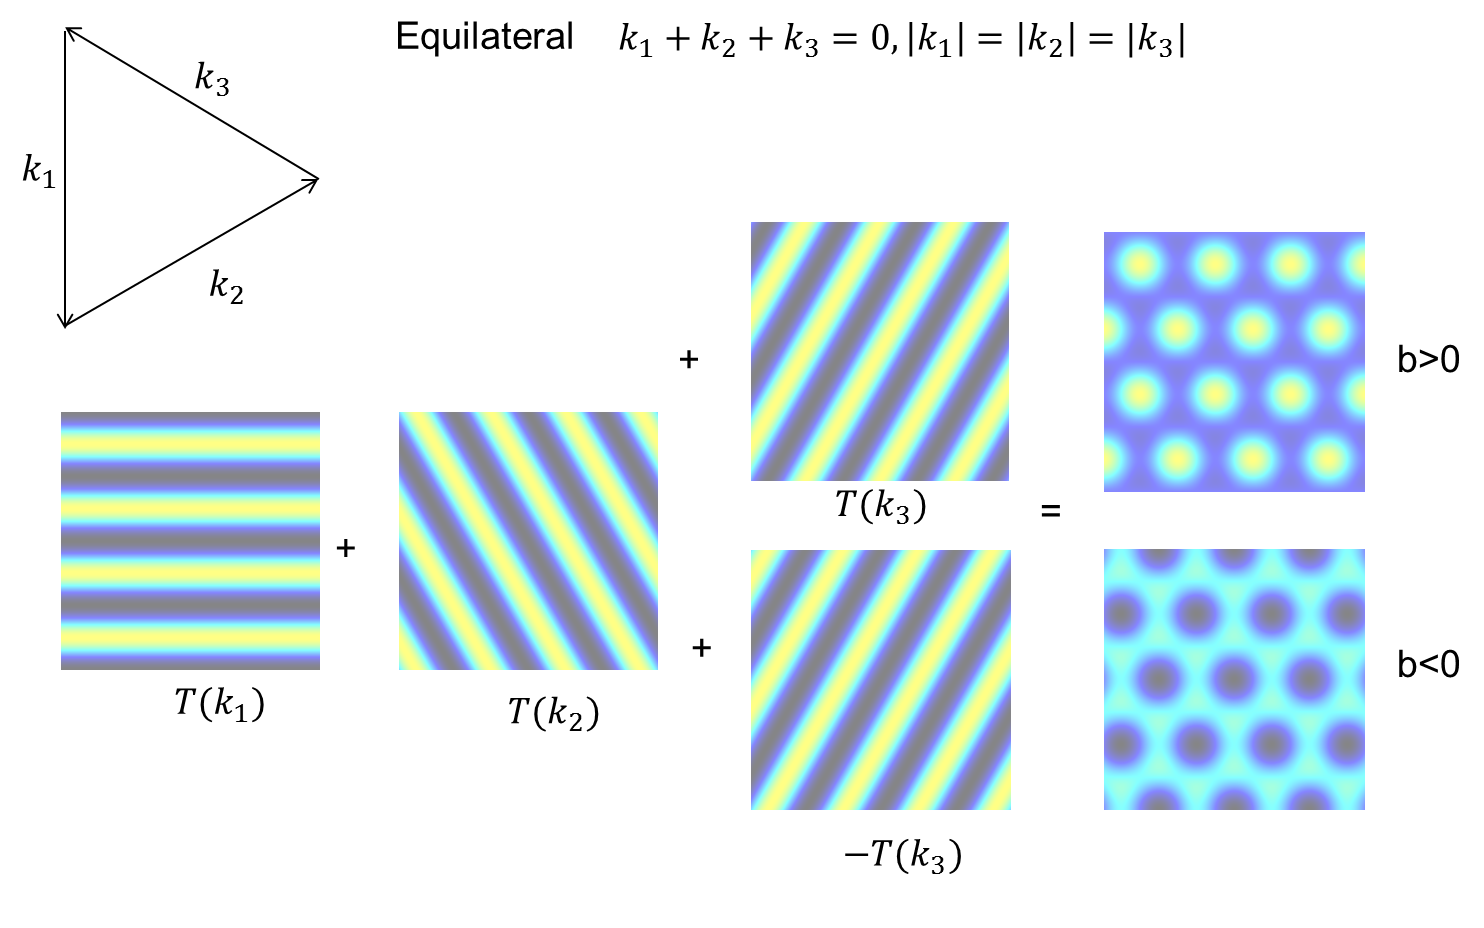
\includegraphics[width=0.8\textwidth]{fig/Equilateral.png}
	\caption{An illustration of a Fourier-space triangle shape and the corresponding real space signature-- in this case the equilateral bispectrum. The field (denoted T here) can be decomposed into plane waves, and the three components that form an equilateral triangle can have different signs relative to each other. This gives an overall sign to bispectrum $b$, to be interpreted as an average probability of which sign is more likely. A positive sign corresponds to the combination of wavevectors being more likely to produce concentrated overdensities surrended by areas of milder underdensity. For a negative equilateral bispectrum, this is the other way round, and one would expect to see on average more concentrated underdensities surrounded by areas with mild overdensity. Please note that these are slices of 3D figures, which extend into the page-- meaning that a positive sign on the bispectrum corresponds to filaments of overdensities surrounded by areas of mild underdensity. Note also that this concerns a statistical quantity only, so while on average one would expect to see more of one type of signature, the observed distribution does not uniformly look like a given real space structure. Figure taken from~\cite{Lewis:2011}}
	\label{fig:realspacesignature}
\end{figure}



\subsubsection{Measurements of the bispectrum}

Most measurements of higher-order correlation functions so far are rather noisy and imprecise, and there is a lack of dedicated analysis tools (e.g. theoretical predictions, estimators, likelihood models) for higher-order statistics compared to the analysis toolkit available for two-point statistics. Forecasts for constraints using the galaxy bispectrum usually assume that the main cosmological parameters are known exactly, and determine expected uncertainty on the bias and/or non-Gaussianity parameters~\cite{Scoccimarro:2003wn,Sefusatti:2007ih,Song:2015gca,Tellarini:2016sgp,Yamauchi:2016wuc,Karagiannis:2018jdt}, which recently got extended to theories of modified gravity~\cite{Yamauchi:2017ibz}. Fisher forecasts using joint galaxy clustering data and CMB data are presented in~\cite{Sefusatti:2006pa}, Other related work has focussed on developing optimal compression algorithms for three-point statistics~\cite{Byun:2017fkz,Gualdi:2018pyw}, and on detecting PNG due to massive spinning particles during the inflationary era~\cite{MoradinezhadDizgah:2018ssw}. Forecasts combining measurements of the galaxy power spectrum and bispectrum to constrain the standard cosmological parameters was done in~\cite{Yankelevich:2018uaz}, which uses the standard Newtonian contributions to the galaxy bispectrum only for signal-to-noise ratio calculations as well as Fisher forecasts. See Figure~\ref{fig:snr_yp} for an example of a forecast for the SNR using the bispectrum.

\begin{figure}[!ht]
	\centering
	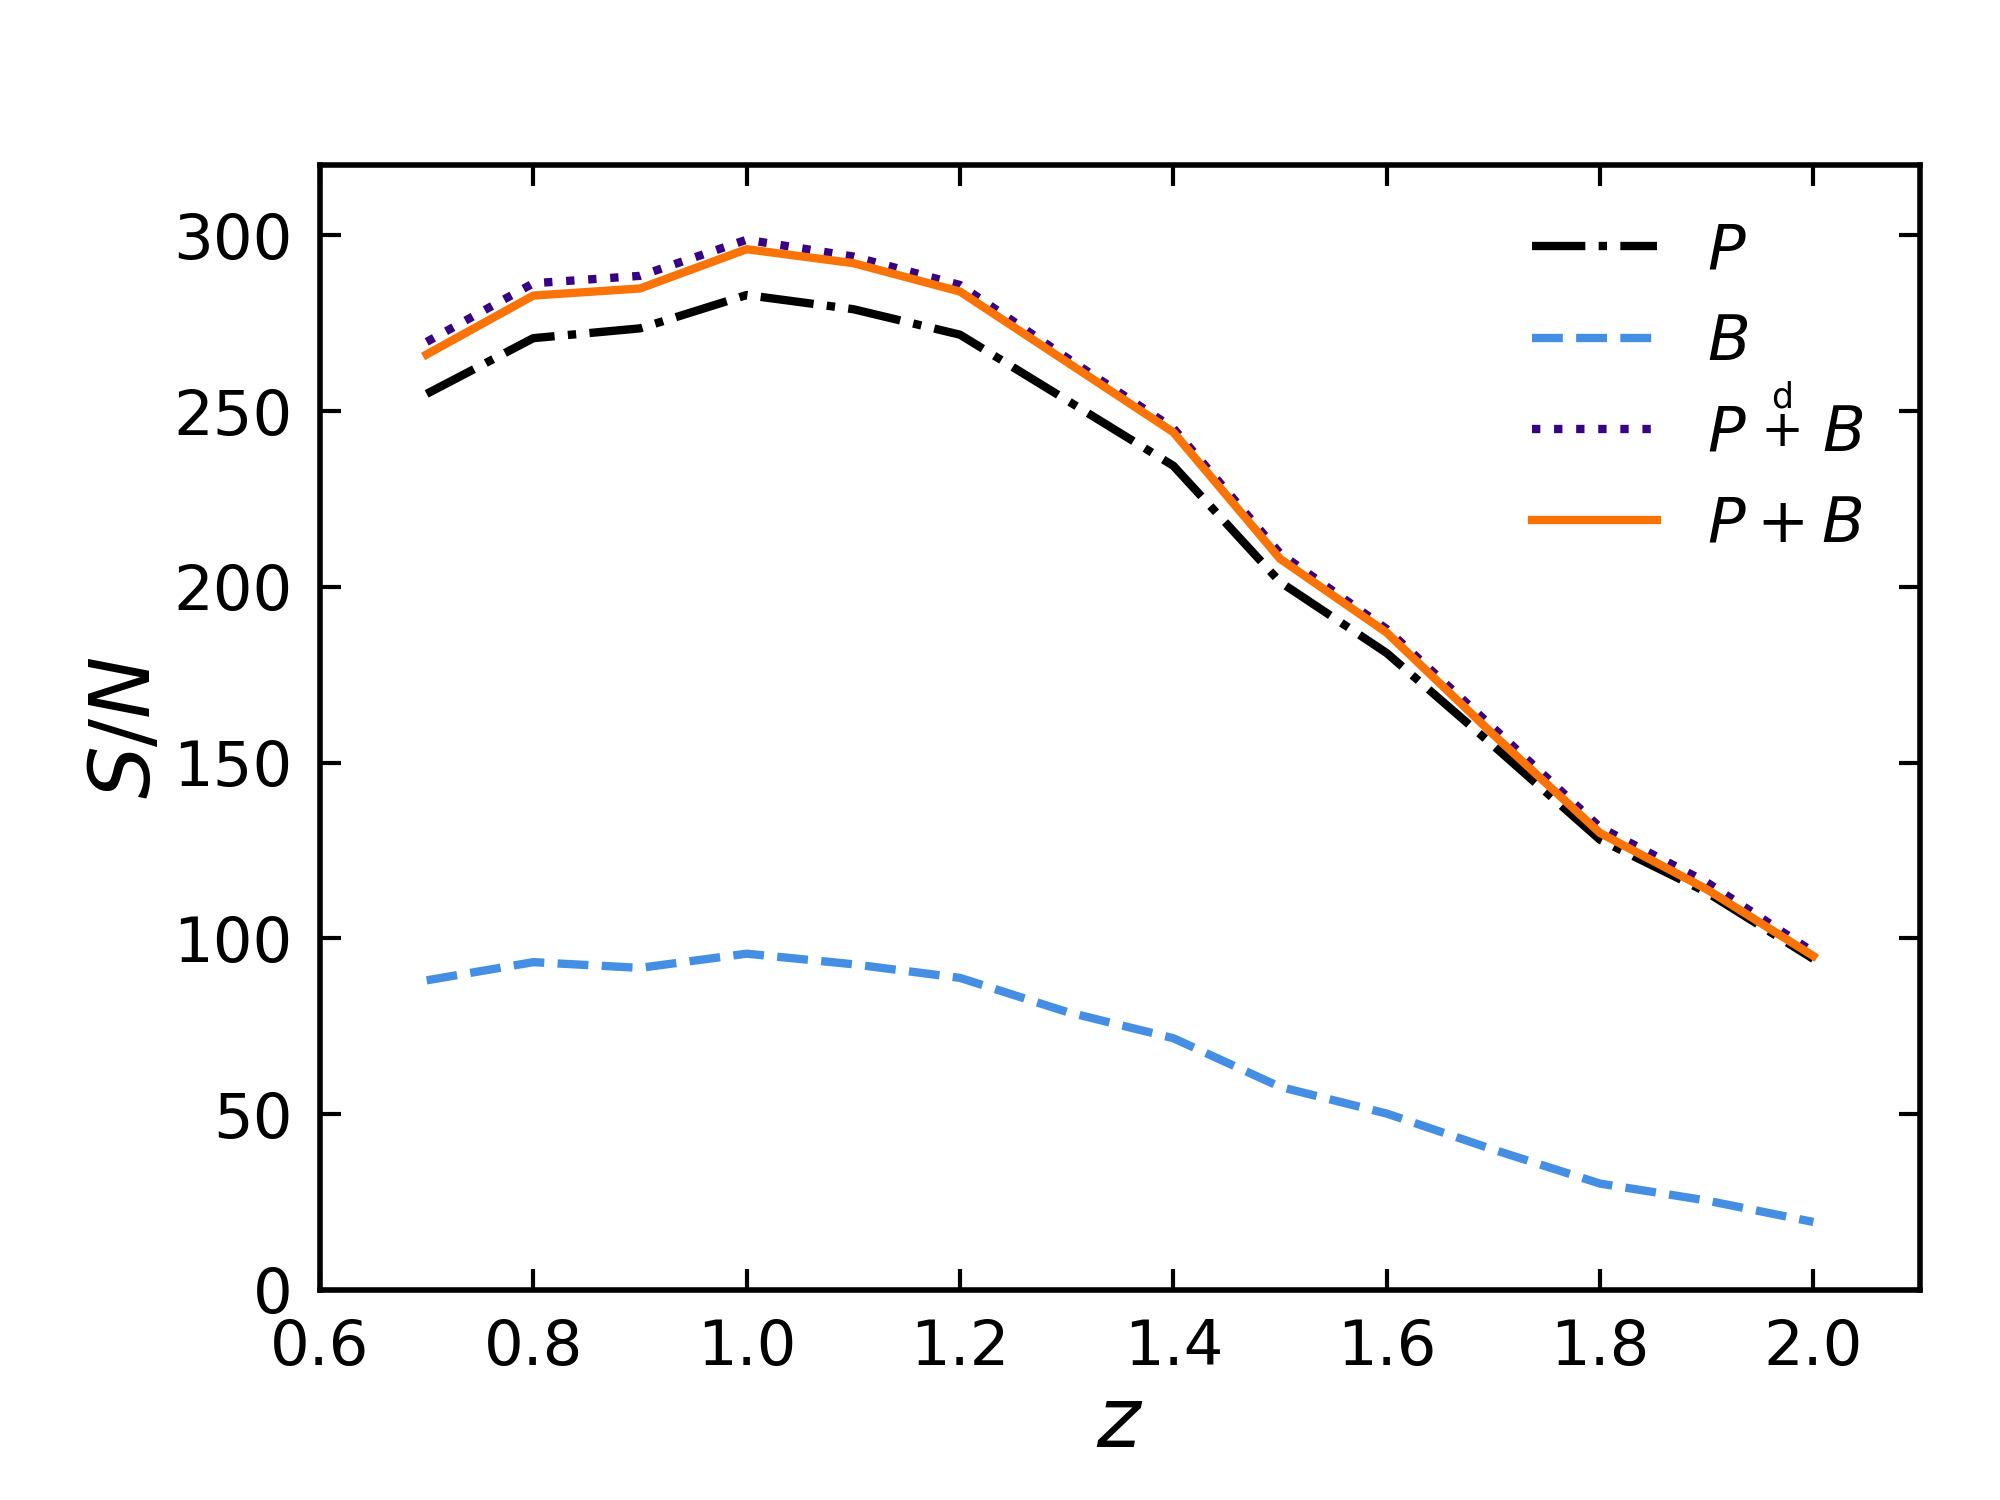
\includegraphics[width=0.7\textwidth]{fig/ypsnr.png}
	\caption{Signal-to-noise ratio for measurements of the galaxy power spectrum and bispectrum in a Euclid-like galaxy survey as a function of redshift $z$, as computed by~\cite{Yankelevich:2018uaz}. Displayed are the SNR for the power spectrum (dot-dashed), bispectrum (dashed). Solid line is the combined SNR, and the SNR computed by neglecting the cross-covariance between the power spectrum and bispectrum is denoted by a dotted line.}
	\label{fig:snr_yp}
\end{figure}

\section{Galaxy bias}
\label{section:galaxybias}

Galaxy bias is the statistical relation between the observed distribution of galaxies and the underlying matter distribution. On scales where the cosmic density fields are quasi-linear, the clustering of galaxies can be described by a perturbative bias expansion. In this formalism, the complicated physics concerning formation of galaxies can be absorbed by a finite set of expanion coefficients known as the bias parameters. In this section we will briefly review the origin of the field and set out the relevant bias models for this thesis. For the majority of this thesis, that is, up to Chapter~\ref{chapter:multipoles}, we use a simple local Gaussian model of galaxy bias. Primordial non-Gaussianity, which we include in Chapter~\ref{chapter:localpng}, introduces a scale-dependence in galaxy bias and hence requires separate treatment. It is worth noting that we consider only PNG of the local type. For a full review of galaxy bias, see~\cite{Desjacques:2016bnm}.

All sorts of galaxy surveys and the resulting statistical studies of the distribution of galaxies ciritally rely on a robust description of the relation between the galaxies and the underlying dark matter. Of course galaxies are not the only tracers of this dark matter distribution, but the term galaxy bias is often used as a convenient term to encompass the biasing of all such tracers. Other examples include, but are not limited to, the Lyman-$\alpha$ forest, and HI intensity mapping-- the latter of which is considered in this thesis along with the more traditional spectroscopic galaxy surveys. 

Roughly speaking, LSS can be divided into two regimes, small non-linear scales, which cannot be described with perturbation theory, and large quasi-linear scales, which can adequately be described by perturbation theory, provided if it is carried out to sufficiently high order. Here we will consider only quasi-linear scales, so that perturbation theory will not break down. On these scales, the complex process of galaxy formation, which is itself far from being understood in detail, can at each order in perturbations and at fixed time, be absorbed into a finite set of parameters called the bias parameters. This is a remarkable result, and relies on the fact that on large scales the formation of structure is almost entirely determined by gravity. 

\subsection{Local-in-mass-density model of galaxy bias}

The simplest example of a local model of galaxy bias is the local-in-mass-density (LIMD) model of galaxy bias. In this model, we assume that dark matter haloes simply correspond to overdensities (i.e. regions above some threshold density $\delta_\mathrm{cr}$).

\begin{figure}[!ht]
	\centering
	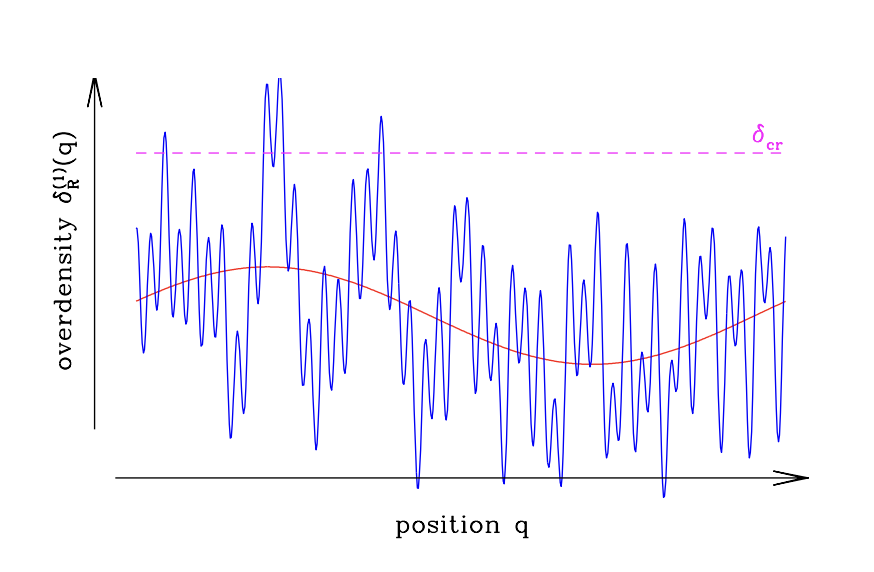
\includegraphics[width=0.8\textwidth]{fig/limdcartoon.png}
	\caption{Illustration of the LIMD model of galaxy bias. The red line indicates a long wavelength perturbation, and the blue line denotes the density field $\delta_R$. The dashed horizontal magenta line shows the critical density $\delta_{\mathrm{cr}}$. Regions of overdensity $\delta_R$ that get pushed above this critical density threshold collapse to form halos in which galaxies are formed.}
	\label{fig:limdcartoon}
\end{figure}

\iffalse
The general form of the LIMD model of galaxy bias is expanding the galaxy overdensity $\delta_g$ in terms of dark matter overdensities with bias coefficients as, 
\begin{equation}
	\delta_g = b_1 \delta + \frac{b_2}{2} \delta^2 + \ldots\,.
\end{equation}

The bias coefficients $b_O$ can be understood to be coefficients of some physical operators $O(\x,\eta)$ in an expansion of the galaxy overdensity, which has the general form,
\begin{equation}
	\delta_g(\x,\eta) = \sum_O b_O(\eta) O(\x,\eta)\,.
\end{equation}
On the scales of interest-- quasi-linear scales,where perturbation theory remains valid, higher order terms in the expansion are successively suppressed, and the expansion converges. Whether such an expansion is performed at initial time (Lagrangian) or at final time (Eulerian) is a matter of choice.

The simplest example of a local bias expansion would be the LIMD bias in Lagrangian space. This bias model is motivated by the spherical collapse approximation to halo formation. A local operator here means any leading local gravitational observable-- this includes but is not limited to the matter density and tidal field. LIMD bias, sometimes called simply `local bias', is a more restricted expansion only in powers of density perturbation $\delta$.

In this simplified model, we assume dark matter halos to simply correspond to overdense regions (i.e. above some threshold density) in Lagrangian space. The observed galaxies reside in these dark matter halos. More specificially, this means that the initial matter density field, which is assumed to be Gaussian and often referred to as the linear density field $\delta^\on$, is extrapolated to some desired reference time using linear growth. 

We will review how the local bias expression in the Newtonian case is derived, and will just quote the results for the more complicated relativistic case when appropriate later on in this thesis. There are a few more things to consider along with the order of the perturbative expansion of the galaxy bias, since there are other factors that play a role in the formation of galaxies. To have a physically motivated definition of galaxy bias, one needs to introduce a physical scale, which denotes some spatial region associated with the process of galaxy formation. Intuitively this means that the number of galaxies formed in a certain region depends on the detailed distribution of the underlying matter-- as well as on other gravitational observables such as tidal fields, which enter our description of galaxy overdensity as tidal bias, as we shall see later on. A final thing to consider is that the naive relation between the galaxy density field $\delta$ and the operators $O$ is deterministic. In reality, one needs to account for some randomness, or stochasticity, since whether or not a galaxy forms in any given location depends on initial conditions on very small scales. The random phases of these scales are not covered by our perturbative bias expansion. Adding this stochasticity, we obtain, 
\begin{equation}
	\delta_g(\x, \eta) = \sum_O b_O(\eta) O(\x,\eta) + \epsilon(\x,\eta) + \sum_O \epsilon_O(\x,\eta) O(\x,\eta)\,, 
\end{equation}
where the random $\epsilon$ and $\epsilon_O$ are uncorrelated with the large-scale perturbations described by the operators $O$, as well as uncorrelated amongst themselves on large scales. Then, their contribution to the total galaxy statistics can be described by a finite set of parameters. 

The LIMD model is based on the simple assumption that the dark matter halos in which galaxies reside simply correspond to overdense regions in Lagrangian space. In order to define the regions `above threshold' which end up collapsing to form halos, we filter the initial density field on a scale corresponding to the spatial region associated with galaxy formation $R$ and call this $\delta_R$. Figure~\ref{fig:limdcartoon} illustrates the density field $\delta_R$ in relation to the critical density threshold $\delta_\mathrm{cr}$.



\fi

\subsection{Scale-dependent bias in the presence of PNG}
Scale-dependent bias in literature can refer to any non-trivial (i.e. $k$-dependent) Fourier-space relation between galaxy overdensity and the underlying dark matter density. Primordial non-Gaussianity generates such a leading non-local term in the bias relation. In this thesis we only consider PNG of the local type. This is defined as a simple form of non-linearity in the primordial curvature perturbation, which is local in configuration space. Usually, these perturbations are expressed in terms of the Bardeen potential $\varphi$. This in turn is directly related to the curvature perturbation in comoving gauge 


\iffalse



\iffalse
The Poisson-gauge number density contrast at first order, $\delta_g^\on$, is related to the dark matter density contrast $\delta_m^\on$ via the galaxy bias. For now we will use a local model of galaxy bias, and we need ot make sure that the definition of scale-independent bias is gauge-independent, and valid on ultra-large scales. The physical definition of scale-independent galaxy bias is in the matter rest-frame (corresponding to the comoving-synchronous C gauge), which since there is no velocity bias on large scales coincides with the galaxy rest-frame~\cite{Challinor:2011bk,Bruni:2011ta,Jeong:2011as}. It then follows that the correct definition between the galaxy and dark matter number density contrasts at first order is, 
\begin{equation}\label{eq:deltagbiasdef}
	\delta_{g\cs}^\on (a, \x) = b_1(a) \delta_{m,\cs}^\on(a,\x)\,.
\end{equation}
The Poisson gauge number density contrast $\delta_g^\on$ is related to the C-gauge number density contrast as~\cite{Challinor:2011bk}, 
\begin{equation}\label{eq:deltagFOPgtoCg}
	\delta_{g}^\on = \delta_{g\cs}^\on + (3 - b_e)\cH v^\on = b_1 \delta_{m\cs}^\on + (3 - b_e) \cH v^\on\,,
\end{equation}
where the velocity potential term ensures that this bias relation is gauge-independent on ultra-large scales. Because of the scale dependence of the velocity potential as given by equation~\eqref{eq:scdepvel}, this term is the relativistic part of the Poisson-gauge number density contrast-- it is suppressed on small scales, and growing on large scales. 

In GR, the Lagrangian frame coincides with the C-gauge~\cite{Villa:2015ppa,Bertacca:2015mca}. There is no unique Eulerian frame, but the total-matter (T) gauge is a convenient choice, because it is related to the C gauge by a purely spatial transformation only such that at first order the galaxy and matter overdensities are the same,~\cite{Bertacca:2015mca}
\begin{align}\label{eq:deltaFOCgtoTg}
	&\delta^\on_{m\cs} = \delta^\on_{m\mathrm{T}}\,,\\
	&\delta^\on_{g\cs} = \delta^\on_{g\mathrm{T}} = b_1 \delta^\on_{m\mathrm{T}}\,.
\end{align}
The second line above defines the Eulerian first-order bias parameter, from which follows that $b_1$ in equation~\eqref{eq:deltagbiasdef} is the Eulerian bias parameter.

Since we require second order in perturbation theory in order to compute the galaxy bispectrum at tree level, we have to extend equation~\eqref{eq:deltagbiasdef} to highter order. To do this, we here use the so-called local-in-mass-density bias model~\cite{Desjacques:2016bnm}, which is the simplest possible model of scale-independent bias we can use. This model assumes that the galaxy number density contrast is a local function of only the matter density contrast. (In chapter~\ref{chapter:localpng}, we introduce local PNG to the bispectrum, in which case we have scale-dependent bias.) Again we need to ensure that the bias coefficients are scale-independent in the C-gauge, which is the galaxy rest frame-- this is to ensure validity of the physical definition of scale-independent bias on ultra-large scales. Starting from a simple expansion in powers of the matter density contrast,
\begin{equation}
	\delta_{g\cs} = b_1 \delta_{m\cs} + \frac{1}{2} b_2 (\delta_{m\cs})^2 + \ldots\,,
\end{equation}
where we suppress the dependence of $b_I \equiv b_I(a,\ln L)$ for brevity-- as done throughout the text. At first order in perturbation theory, the above expression recovers the first-order relation given by equation~\eqref{eq:deltagbiasdef} as expected. At second order we have, 
\begin{equation}\label{eq:biasCgauge}
	\delta^\tw_{m\cs} = b_1 \delta^\tw_{m\cs} + b_2 (\delta^\on_{m\cs})^2\,,
\end{equation}
where we have omitted the term $- b_2 \langle (\delta^\on_{m\cs})^2 \rangle$ on the right hand side for convenience.

At second order, the C-gauge and T-gauge matter overdensities are related as~\cite{Bertacca:2015mca,Villa:2015ppa}, 
\begin{equation}
	\delta_{m\mathrm{T}}^\tw = \delta_{m\cs}^\tw + 2 \left[ \partial_i \delta_{m\cs}^\on \right] \nabla^{-2} \partial^i \delta_{m\cs}^\on\,,
\end{equation}
where $-2\nabla^{-2} \partial^i \delta_{m\cs}^\on$ is a gauge generator. The gauge transformation from comoving-synchronous to total-matter gauge is purely spatial, which means that the above relation applies to the galaxy number counts too, 
\begin{equation}
	\delta_{g\mathrm{T}}^\tw = \delta_{g\cs}^\tw + 2 \left[ \partial_i \delta_{g\cs}^\on \right] \nabla^{-2} \partial^i \delta_{g\cs}^\on\,.
\end{equation}
From the above relations, we can obtain the T-gauge galaxy number count density in terms of T-gauge matter density, 
\begin{align}
	&\delta_{g\mathrm{T}}^\tw = b_1 \delta_{m\cs}^\tw + b_2 (\delta_{m\cs}^\on)^2 + 2 b_1 \left[\partial_i \delta_{m\cs}^\on \right] \nabla^{-2} \partial^i \delta_{m\cs}^\on \\
	& \hphantom{\delta_{g\mathrm{T}}^\tw } = b_1 \left[ \delta_{m\cs}^\tw + 2 (\partial_i \delta_{m\mathrm{T}}^\on) \nabla^{-2} \partial^i \delta_{m\cs}^\on \right] + b_2 (\delta_{m\cs}^\on)^2 \\
	& \Rightarrow \delta_{g\mathrm{T}}^\tw = b_1 \delta_{m\mathrm{T}}^\tw + b_2 (\delta_{m\mathrm{T}}^\on)^2 \label{eq:biasTgauge} \,.
\end{align}

Comparing equations~\eqref{eq:biasCgauge} and~\eqref{eq:biasTgauge}, it is clear that local-in-mass-density and scale-independent bias in C- and T-gauge are equivalent up to second order in perturbation theory and have the same Eulerian bias coefficients. 

The Poisson gauge expression for overdensity can more conveniently be expressed in the T gauge than in the C gauge, and hence we will choose the total-matter gauge to express $\delta_g$. This expression is as follows~\cite{Jolicoeur:2017nyt},
\begin{align}
	\delta_g^\tw =& \delta_{g\mathrm{T}}^\tw + (3 - b_e)\cH v^\tw + 2 (3 - b_e) \cH v^\on \delta_{g\mathrm{T}}^\on - 2 v^\on \delta_{g\mathrm{T}}'^\on \nonumber \\
	&+ \left[ (b_e - 3)\cH' + b_e \cH + (b_e -3)^2 \cH^2  \right] \left[ v^\on \right]^2 + (b_e - 3) \cH v^\on v^{\on\prime} \nonumber \\
	& - (b_e - 3) \cH \nabla^{-2} \left[ v^\on \nabla^2 v^{\on\prime} - v^{\on\prime} \nabla^2 v^\on - 6 \partial_i \Phi^\on \partial^i v^\on - 6 \Phi^\on \nabla^2 v^\on \right] \,.
\end{align}
From this, using relations between the T-gauge galaxy density contrast and matter contrast, we obtain the final expression for the Poisson-gauge galaxy density contrast in the simple local-in-mass-density bias model, 
\begin{align}
	\delta_g^\tw =& b_1 \delta_{m\mathrm{T}}^\tw + b_2 (\delta_{m\mathrm{T}}^\on )^2 + \left[ (b_e - 3)\cH' + b_e \cH + (b_e -3)^2 \cH^2 \right] [v^\on]^2 \nonumber \\
	&+ (b_e - 3) \cH v^\on v^{\on \prime} + 2 b_1 (3 - b_e) \cH v^\on \delta_{m\mathrm{T}}^\on - 2 v^\on \left[ b_1 \delta_{m\mathrm{T}}^{\on \prime} + b_1' \delta_{m\mathrm{T}}^\on \right] \nonumber \\
	& + (3 - b_e) \cH \nabla^{-2} \left[ v^\on \nabla^2 v^{\on \prime} - v^{\on \prime} \nabla^2 v^\on - 6 \partial_i \Phi^2 \partial^i v^\on - 6 \Phi^\on \nabla^2 v^\on \right]\,.
\end{align}
In the above equation, the velocity and metric potentials ensure that there is gauge-independence on ultra-large scales. 
\fi
\fi
\section{Primordial non-Gaussianity}

Types of primodial non-Gaussianity in the bispectrum, their signatures on various scales, scale dependence it introduces in the clustering bias etc. 

Also gotta mention how formation of structure itself gives rise to non-Gaussianity in the universe which can mimic fnl on large scales, include some pictures from like sheean's papers etc-- showing the bias from a Gaussian treatment.

The rest of this thesis is organised as follows. In Chapter~\ref{chapter:dipole}, we introduce the lowest order (i.e. least suppressed) relativistic corrections to the bispectrum and consider how they affect the amplitude of the bispectrum. These leading-order relativistic corrections give rise to a local dipole with respect to the observer's line-of-sight, which is absent in the purely Newtonian picture. The amplitude of this dipole, which if detected would be a smoking-gun signal for relativistic corrections, is even on equality scales about 10\% of that of the monopole (at redshift $z = 1$). This implies that the dipole of the bispectrum is a unique signature of GR on cosmological scales. In Chapter~\ref{chapter:detect}, we make an estimate for the detectability of such a relativistic signal in next-generation spectroscopic and intensity mapping surveys. For a Stage IV spectroscopic survey similar to \textit{Euclid}, we find that the signal-to-noise ratio for these leading order effects is of $\sim 17$, while the 21cm intensity mapping surveys suffer from foreground and beam effects-- we forecast a marginally detecable SNR of $\sim 6$ for SKA1 and $\sim 5$ for HIRAX. Then, Chapter~\ref{chapter:ho} summarises past work on adding local relativistic corrections at all orders of $\cH/k$ to the bispectrum, and a fully analytic multipole expansion with relevant numerical analyses for future surveys is presented in Chapter~\ref{chapter:multipoles}. The relativistic bispectrum generates non-zero multipoles for both even and odd multipole number $\ell$, where the odd multipoles are induced by relativistic effects only. Finally, we expand the theoretical description of the Fourier-space galaxy bispectrum by adding local primordial non-Gaussianity in Chapter~\ref{chapter:localpng}. This allows for better separation of the relativistic signature and biasing due to the presence of PNG-- we find that the bias from using a Newtonian analysis of the squeezed bispectrum could be as large as $\Delta f_\nl \sim 5$ for a Stage IV H$\alpha$ survey. 